% !TEX TS-program = pdflatex
% !TEX encoding = UTF-8 Unicode

% This is a simple template for a LaTeX document using the "article" class.
% See "book", "report", "letter" for other types of document.

\documentclass[11pt]{IEEEtran} % use larger type; default would be 10pt

\usepackage[utf8]{inputenc} % set input encoding (not needed with XeLaTeX)

%%% Examples of Article customizations
% These packages are optional, depending whether you want the features they provide.
% See the LaTeX Companion or other references for full information.



\usepackage{graphicx} % support the \includegraphics command and options

% \usepackage[parfill]{parskip} % Activate to begin paragraphs with an empty line rather than an indent

%%% PACKAGES
\usepackage{url}
\usepackage{booktabs} % for much better looking tables
\usepackage{array} % for better arrays (eg matrices) in maths
\usepackage{paralist} % very flexible & customisable lists (eg. enumerate/itemize, etc.)
\usepackage{verbatim} % adds environment for commenting out blocks of text & for better verbatim
\usepackage{subfig} % make it possible to include more than one captioned figure/table in a single float
\usepackage{algorithm} 
\usepackage{algorithmic}
\usepackage[firstpage]{draftwatermark}


% These packages are all incorporated in the memoir class to one degree or another...

%%% HEADERS & FOOTERS
%\usepackage{fancyhdr} % This should be set AFTER setting up the page geometry
%\pagestyle{fancy} % options: empty , plain , fancy
%\renewcommand{\headrulewidth}{0pt} % customise the layout...
%\lhead{}\chead{}\rhead{}
%\lfoot{}\cfoot{\thepage}\rfoot{}

%%% END Article customizations

%%% The "real" document content comes below...

\title{Distributed Decentralized Domain Name Service}
\author{
Brendan Benshoof \qquad Andrew Rosen  \\Department of Computer Science, Georgia State University\\ 34 Peachtree St NW \\ Atlanta, Georgia 30303\\  bbenshoof@cs.gsu.edu \qquad rosen@cs.gsu.edu }
%\date{} % Activate to display a given date or no date (if empty),
         % otherwise the current date is printed 

\begin{document}
\maketitle

\begin{abstract}

We present D$^{3}$NS, a system to replace the current top level DNS system and certificate authorities, offering increased scalability, security and robustness. 

D$^{3}$NS is based on a distributed hash table and utilizes a domain name ownership system based on the Bitcoin blockchain.  It addresses previous criticism that a DHT would not suffice as a DNS replacement. 

D$^{3}$NS provides solutions to current DNS vulnerabilities such as DDOS attacks, DNS spoofing and censorship by local governments. D$^{3}$NS eliminates the need for certificate authorities by providing a decentralized authenticated record of domain name ownership. Unlike previous DNS replacement proposals, D$^{3}$NS is reverse compatible with DNS and allows for incremental implementation within the current system.

%We have created a system to replace the top level of the Domain Name system. The goal is to replace the top level of DNS with a network of authoratative name servers sharing their DNS records over a DHT.

%We attempt to address the core problem posed by centralized trusted third parties. Specifically that centralized authorities are a single point of failure for trust. We seek to diffuse the responsibility of these system such that abuse of trust is more difficult.

%It is reverse compatible with traditional DNS and entirely transparent to end users.


\end{abstract}


\section{Introduction}
The Domain Name System, commonly referred to as DNS \cite{mockapetris2003rfc} \cite{mockapetris2004rfc}, is a fundamental component of the Internet.  DNS maps memorable names to the numerical IP addresses used by computers to communicate over IP. 

%cut this for conference?
Two recent events in the United states have brought DNS to the forefront of networking and security research.  First is recent legislation proposed in the US House of Representatives and US Senate. The Stop Online Piracy Act (SOPA) \cite{sopa} and PROTECT IP Act (PIPA) \cite{pipa} were both introduced in 2011.  There were numerous aspects to both bills, but essential to both was that DNS servers located in the US would be required filter DNS records on demand, essentially fracturing the DNS system.  There would be no guarantee that DNS could serve the same information to two different users.

More recent are the leaks of classified information elucidating the extent of the NSA's spying capabilities. These leaks have raised questions about the security of SSL and TLS, as well as the level of trust that users place in certificate authorities.


These types of threats to DNS, along with security concerns, were not considered when designing the protocol, but DNS is too widely used and too integrated with the Internet as a whole to be replaced. Extensions such as DNSSEC \cite{blacka2013clarifications} add authentication and data integrity, but do not alter the fundamental architecture of the DNS network.


There have been many explorations and attempts \cite{cox} \cite{pappas} \cite{ramasubramanian2004design} to propose a DNS system based on a distributed hash table (DHT) cite{chord}. We extend on those papers by implementing a DHT which minimizes latency distance rather than hop distance and implementing a shared record of ownership based on recent developments in cryptocurrency \cite{namecoin} \cite{bitcoin}.


This paper proposes the Distributed Decentralized Domain Name Service, or D$^{3}$NS.  D$^{3}$NS is a completely decentralized Domain Name Service operating over a DHT.  D$^{3}$NS does not replace the DNS protocol, but rather adds robustness to the architecture as a whole.  Internally, D$^3$NS signs all DNS records using public/private keys, providing additional security internal to the DNS system.

We show that D$^{3}$NS addresses the objections to a decentralized DNS system posed by Cox et al \cite{cox}, specifically: dramatically reducing latency compared to other DHT systems, retaining the extensibility of the original DNS system, and changing the intended scope of use to address incentive issues. We show D$^{3}$NS allows for new authentication methods and a means of decentralized proof of ownership beyond that of Cox et al's work. 


The rest of the paper is consists of the following sections.  Section II gives an overview of DNS and identifies prior research in the area of distributed DNS.  Section III defines the various components of D$^3$NS.  Section IV covers the modified blockchain used for record authentication in D$^3$NS.  Section V presents VHash, a DHT that we designed for D$^3$NS.  Section VI details our implementation of D$^3$NS and  we discuss our conclusions and future work in Section VIII.


\section{Background}

This paper is intended to address concerns raised by Cox et al \cite{cox} and propose a viable decentralized DNS replacement utilizing a DHT. Our proposed improvements on the DNS alternative presented by Cox et al are fully reverse compatible with the current hierarchical DNS system and provides a shared, authenticated public record that allows for DNSSEC style authentication.

\subsection{DNS Overview}

DNS queries proceed recursively through the DNS hierarchy, beginning with a query to a root server, which then yields a record for a server for the requested top level domain.  This server then directs the request to another DNS server responsible for the domain under that, which yields an answer or another DNS server, which is queried in the same manner.

One of the key concepts of the DNS architecture is that no matter which servers end up being queried, a user can expect to receive a record consistent with what the rest of the DNS system will serve for that particular request.
\
Multiple recent legislative motions reflect DNS's weakness to be influenced by local government intervention \cite{sopa} \cite{lemley2011don} \cite{crocker2011security}.

These bills would have required that servers maintained in the US filter specified domain names, preventing users from obtaining the correct IP address for the domain name in question. Multiple governments have been noted to preform systematic attacks on DNS queries \cite{inject}. This filtering is incompatable with the DNS Security Extensions (DNSSEC) \cite{crocker2011security} and DNS's intended usage. 

The mandated DNS filtering would possibly drive users to unregulated DNS servers, which would create more attack vectors.


\subsection{Related Work}
Cox et al devised a distributed DNS using Chord \cite{chord} as the storage medium for DNS records, which they called Distributed DNS (DDNS). They examined the possibility of extending DNSSEC with new options for storing keys in the DHT. They encountered the then unsolved problem of proof-of-ownership \cite{bitcoin} for domain names and found no means of enhancing security. 

They noted that the overlay topology of a DHT such as Chord did not take into account latency optimization and thus DNS was not a viable application of a DHT due to significantly greater latency. They also pointed out several possible improvements as a result of using a DHT, namely increased robustness, an auto-balancing structure, resistance to both DDOS attacks and packet injection based DNS spoofing.


Cox et al considered the optimization and security problems solvable, but they postulated that two issues rendered the system unviable. First, they intended that DDNS would replace all DNS servers and traffic, which removed extensibility and customizability of the original DNS protocol. Second, because they considered replacing the entire DNS system rather than a meaningful subset, they presented a question of incentive. What incentivized companies to support the new system where their servers had to share the load of other companies traffic?  What would stop them from holding only their content, while rejecting any additional responsibility assigned to it?
 
 
D$^3$NS addresses both of the raised issues. We utilize a side channel method of confirming domain named ownership via a blockchain \cite{namecoin} to enable DNSSEC style security at all layers of the network. We propose a DHT structure which allows for minimum latency optimization. Our system aims only to replace authoritative Top Level Domain servers currently managed by registrars, where most records are simpley a forward to an authoritative DNS server managed by the domain owner, rather than replacing all levels of DNS. This limiting of scope allows us to continue to take advantage of DNS extensions and as places responsibility of managing the network with those who have an incentive for its continued functioning.



\section{D$^{3}$NS}
D$^{3}$NS has logically discrete components which provide DNS efficient record storage, domain name ownership management and verification, and DNS backwards compatitibility, all of which may be modularly replaced or have individual optimizations. D$^{3}$NS uses a DHT to store DNS records in a distributed fashion and a blockchain and Namecoin\cite{namecoin} analog to manage domain name ownership.  D$^{3}$NS utilizes public and private key encryption for signing and verifying records.


\subsection{Distributed Hash Table}
Our implementation is not strictly specific to any particular distributed hash table.  We examined using Chord \cite{chord} with DNS, similar to DDNS \cite{cox}.  However, Chord’s unidirectional ring overlay topology does not take actual network topology into account and using it for a global scale system is not viable because messages will be routed very inefficiently. D$^3$NS requires a DHT which allows the routing overlay to be optimized to the network topology and conditions in real time.

As a result we chose to develop a prototype DHT to meet this requirement to act as backend to our DNS system called Vhash. Vhash is built on the idea of an "overlay space" which is a $d$-dimensional unit cube which wraps around the edges in a toroidal fashion. Each record in the DHT is assigned a location in that space. Each node is assigned a location and is responsible for records to which it is the closest node. The variable dimensionality is allowed so that problems can be embedded into the space with relative ease and records can be assigned locations which have meaning concerning the problem in which they are a part. This way, records that are close to each other in the problem formulation are close to each other in the DHT and are likely hosted on the same node. This offers speedup for many distributed algorithms which require traversal of data.



\subsection{DNS frontend}
Because this system is intended to be reverse compatible with the existing DNS protocol, we serve the data provided by the DHT after it has been authenticated by the block chain to other DNS servers or clients. DNS nodes incorporated into the D$^3$NS system will not request data from other DNS servers and will only exchange data via the DHT.


\section{Blockchain}
We use a tool called a \emph{blockchain} for maintaining and  authenticating our DNS records.  Blockchains have their roots in the cryptocurrency Bitcoin \cite{bitcoin}, where it is used to authenticate financial transactions and verify account balances.  While there have been similar attempts to leverage Bitcoin's mechanisms extend DNS \cite{namecoin}, they have been strictly tied to the concept of currency and not yet academically explored.

\subsection{Blockchains in Bitcoin}
Bitcoin is a decentralized electronic currency. 
Here we are particularly concerned with Bitcoin's blockchain. Bitcoin's blockchain consists of a shared authenticatable transaction record \cite{namecoin}  \cite{bitcoin} .


\begin{figure}
    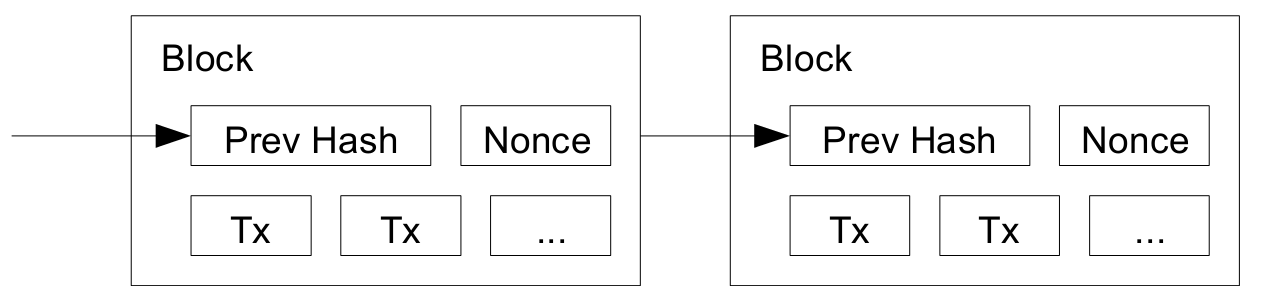
\includegraphics[width=\linewidth]{blockchain}
    \caption{A section of the blockchain as defined by Bitcoin \cite{bitcoin}.}
    \label{blockchain}
\end{figure}


Bitcoin's blockchain is essentially a shared ledger.  The blockchain (Figure \ref{blockchain}) is a record of every single transaction made using the Bitcoin. Each transaction refers to  a previous transaction, indicating the funds handled by the new transaction are in fact owned by the user initiating the transaction. The record is validated by traversing the tree of transactions and marking the referenced transactions as used. A valid blockchain has all non-leaf node transactions marked as used only once.


Transactions are grouped together and verified in a \emph{block}, which are linked together in a chain.  Each block in the chain is a series of transactions published during the time it takes to generate that block. The process of authenticating these transactions and generating a new block is called mining (Algorithm \ref{mining}).  Mining a block is analogous to the concept of gold mining, as the incentive for successfully mining a block is a large sum of new bitcoins.  

A block is mined by generating a nonce field such that the hash of the entire block is less than a global difficulty value. This difficulty sets the rate at which new blocks are mined and is adjusted in reference to rate of mining \footnote{Bitcoin adjusts the difficulty rate every 2016 blocks, such that the network will then mine a block every ten minutes on average \cite{bitdiff}}.  When a block is mined, it is transmitted to the network and each transaction in it is validated by each peer. The network will then work on mining the next block.

\begin{algorithm}
\caption{Blockchain mining}
\label{mining}
\begin{algorithmic}[1]  % the number is how many 
\STATE Given previous Block $B_{-1}$
\STATE Given New Transaction Set $T$
\STATE Given Difficulty $D$
\STATE Given Reward destination $R$
\STATE New Block $B_0$ = $HASH(B_{-1})|T|R|Timestamp$
\STATE Block Attempt $b$ = $B_0|Nonce$
\WHILE {$HASH(b) > D$}
	\STATE Block Attempt $b$ = $B_0|Nonce$
\ENDWHILE
\STATE Propogate $b$ as next block
\end{algorithmic}
\end{algorithm}


\subsection{Using the Blockchain to validate DNS records}
We utilize the transaction record of Bitcoin to record ownership of domain names. Rather than rewarding miners with currency,  the reward and incentive for mining is a record that allots the miner the right to claim a domain name.  


\begin{algorithm}
\caption{Blockchain Transaction Validation}
\label{validation}
\begin{algorithmic}[1]  % the number is how many 
\STATE A new transaction $t$ consists of: Award domain $D$ to user $U$ with proof reference $P$ and signature $S$
\STATE The transaction set $T$ is the set of all transactions considered valid
\IF{$P$ is not marked used}
	\IF{owner indicated in $P$ matches signature $S$}
		\IF{$D$ matches domain referenced in $P$}
    		\STATE Mark $P$ as used
            \STATE Consider $t$ valid
        \ELSE
         	\IF{$P$ is a mining reward}
            	\STATE $P$ is an unclaimed mining reward
                \IF{$D$ is not yet claimed}
                	\STATE Mark $P$ as used
                    \STATE Mark $D$ as claimed
                    \STATE Consider $t$ valid
                \ENDIF
			\ENDIF
         \ENDIF
    \ENDIF
\ENDIF
\end{algorithmic}
\end{algorithm}

The transactions in each block indicate miners claiming a new domain or the transfer of domain ownership. Claims of new domains are validated by a reference to an unclaimed mining reward owned by the claiming user. Transfers are validated by a pointer to an unused previous transfer record or claim record indicating ownership by the transferring party. This way every domain name in the system can be associated with the owner's public key. New domains can be claimed and old domains can be transfered between owners.
Algorithm \ref{validation} shows the process for validating transactions using the blockchain.







\subsection{Using a Blockchain to Replace Certificate Authority}
The shared record of the blockchain allows any participant in the mining network to act as a trusted third party to clients. This way, trust is not centralized at a single point of failure. 

Internally, members of the DHT are also members of the blockchain network (as it is convenient to use the DHT overlay as the Blockchain network overlay) and thus all records pushed to the DHT and retrieved records can be confirmed as legitimate before transmission to the end user. This limits the viability of replay or injection based attacks.




\section{VHash}
VHash was created to allow for spacial representations to be mapped to hash locations, a feature lacking in many current distributed hash tables.  In particular, we aimed to construct a mechanism for creating a more efficient global scale DHT built on a minimal latency overlay. Rather than focus on minimizing the amount of hops required to travel from point to point we wish to minimize the time required for a message to reach its recipient. VHash actually has a worse worst case hop distance ($O(\sqrt[d]{n})$) than other comparable distributed hash tables ($O(lg(n))$). However, VHash can route messages as quickly as possible rather than traveling over a grand tour that an overlay network may describe in the real world.

The naive method of doing so is to assign coordinates to servers based on the geographic location of nodes. More complex approaches would approximate a minimum latency space based on inter-node latency. VHash can be considered  a generalized extension of VoroNet \cite{voronet}.  %Why is Voronet not okay and why is VHash
Algorithm \ref{latency} describes the process for performing a minimum latency embedding using VHash.

%The intent is that meaning can be ascribed to locations in the DHT and facilitate more efficent function. 
%Specifically in this example we seek to build a minimal latency overlay network for the DHT so a global scale DHT is viable and efficent. 








\begin{algorithm}
\caption{Vhash Minimum Latency Embedding}
\label{latency}
\begin{algorithmic}[1]  % the number is how many 
	\STATE $d$ is the dimensions of the hash space
    \STATE seed the space with $d+1$ nodes at random locations
   	\STATE A node $n$ wishes to join the network
    \STATE $n$ pings a random subset of peers to find latencies $L$
    \STATE Normalize $L$ onto (0.0,1.0) to yield $L_N$
    \STATE Choose position $p$ such that $$\sum\limits_{i\in peers}(L_N[i]-dist(p,i))^2$$ is minimized
    \STATE Re-evaluate location periodically
\end{algorithmic}
\end{algorithm}







\subsection{Toroidal Distance Equation}

Given two vector locations $\vec{a}$ and $\vec{b}$ on a  $d$ dimensional unit toroidal hypercube:
\[ distance = \sqrt[|d|]{\sum\limits_{i\in d} (\min(|\vec{a}_i-\vec{b}_i|,1.0-|\vec{a}_i-\vec{b}_i|))^2}\]

\subsection{Mechanism}
VHash maps nodes to a $d$ dimension toroidal unit space overlay. This is essentially a hypercube with wrapping edges. The toroidal property makes visualization difficult but allows for a space without a sparse edge, as all nodes can translate the space such that they are at the center of the space.  In effect, each node views itself at the center of the graph.

VHash nodes are responsible for the address space defined by their Voronoi region. This region is defined by a list of peer nodes maintained by the node. A minimum list of peers is maintained such that the node's Voronoi region is well defined. The links connecting the node to its peers correspond to the links of a Delaunay Triangulation.  One such possible network is shown on Figure \ref{churninit}.


\begin{figure}
    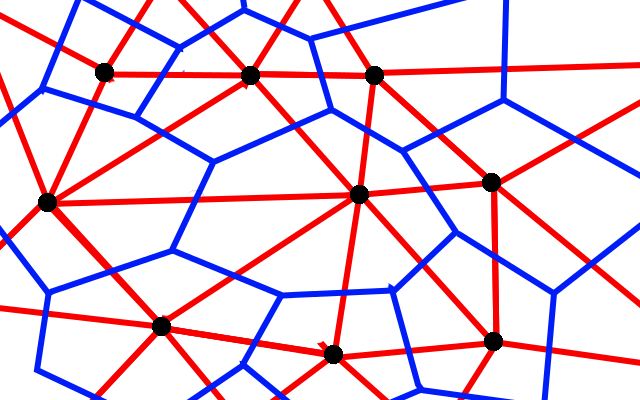
\includegraphics[width=\linewidth]{voronoi-churn2}
    \caption{The starting network topology.  The blue lines demark the Voronoi edges, while the red lines connecting the nodes correspond to the Delaunay Triangulation edges and one-hop connections.}
    \label{churninit}
\end{figure}

\subsection{Relation to Voronoi Diagrams and Delaunay Triangulation}

VHash does not strictly solve Voronoi diagrams \cite{voronoi}, as the toroidal nature of the space preclude the traditional means of solving for Voronoi regions. However, VHash's peer management approximates a topology with similar properties. 
%Rather than attempt to calculate the Voronoi region of each node, it simply filters locations, assigning responsibility to the nearest node. 
An online algorithm (Algorithm \ref{peer} maintains the set of peers defining the node's voronoi region. The set of peers required to define a node's Voronoi Region corresponds to a solution to the dual Delaunay Triangulation.



\begin{algorithm}
\caption{VHash Greedy Peer Selection}
\label{peer}
\begin{algorithmic}[1]  % the number is how many 
	\STATE $Candiates$ is the set of candidate peers
    \STATE $Peers$ is the set of this node's peers
    \STATE $Canidates$ is sorted by each node's closeness to this node
    \STATE The closest member of $Canidates$ is popped and added to $Peers$
    \FORALL{$n$ in $Canidates$}
    	\STATE $c$ is the midpoint between this node and $n$
        \IF{Any node in $Peers$ is closer to $c$ than this node}
        	\STATE reject $n$ as a peer
        \ELSE
        	\STATE Add $n$ to $Peers$
        \ENDIF
    \ENDFOR
\end{algorithmic}
\end{algorithm}


\subsection{Messages}
Maintenance and joining are handled by a simple periodic mechanism. A notification message consisting of a node's information and active peers is the only maintenance message. All messages have a destination hash location which is used to route them to the proper server. This destination can be the hash location of a particular node or the location of a desired record or service.  The message is received by the node responsible for the location. Services running on the DHT define their own message contents, such as commands to store and retrieve data.

\subsection{Message Routing}
Messages are routed over the overlay network using a simple algorithm ( Algorithm \ref{routing}). 
When routing a message to an arbitrary location, a node calculates who's voronoi region the message's destination is in amongst the itself and its peers. If the destination falls within its own region, then it is responsible and handles the message accordingly. Otherwise, the node forwards the message to the closest peer to the destination location. This process describes a pre-computed and cached A* routing  algorithm \cite{astar} . 

\begin{algorithm}
\caption{Vhash Routing}
\label{routing}
\begin{algorithmic}[1]  % the number is how many 
	\STATE $P_0$ is this node's set of peers
    \STATE $N$ is this node
	\STATE $m$ is a message addressed for $L$
    \STATE $Forwards$ is the set $P_0\cup{}N$
    \STATE find $C$: member of $Forwards$ which has the shortest distance to $L$
    \IF{$C$ is $N$}
    	\STATE $N$ is the responsible party.
        \STATE Handle $m$
    \ELSE
    	\STATE Forward $m$ to $C$ for handling or further routing
    \ENDIF
\end{algorithmic}
\end{algorithm}

\subsection{Joining and Maintenance}
Joining the network is a straightforward process. A new node first learns the location of at least one member of the network to join. The joining node then choses a location in the hash space either at random or based on a problem formulation (for example, based on geographic location or latency information).

After choosing a location, the joining node sends a "join" message to its own location via the known node.
The message is forwarded to the current owner of that location who can be considered the "parent" node.
The parent node immediately replies with a maintenance message containing its full peer list. This message is sent to the joining node, who then uses this to begin defining the space it is responsible for. 

The joining node's initial peers are a subset of the parent and the parent's peers. The parent adds the new node to its own peer list and removes all his peers occluded by the new node.  Then regular maintenance propagates the new node's information and repairs the overlay topology.  This process is described by Algorithm \ref{join}.

\begin{algorithm}
\caption{Vhash Join}
\label{join}
\begin{algorithmic}[1]  % the number is how many 
\STATE new node $N$ wishes to join and has location $L$
\STATE $N$ knows node $x$ to be a member of the network
\STATE $N$ sends a request to join, addressed to $L$ via $x$
\STATE node $Parent$ is responsible for location $L$ and receives the join message
\STATE $Parent$ sends to $N$ its own location and list of peers
\STATE $Parent$ integrates $N$ into its peer set
\STATE $N$ builds its peer list from $N$ and its peers
\STATE regular maintenance updates other peers
\end{algorithmic}
\end{algorithm}


Each node in the network performs maintenance periodically by a maintenance message to its peers. The maintenance message consists of the node's information and the information on that node's peer list. When a maintenance message is received, the receiving node considers the listed nodes as candidates for its own peer list and removes any occluded nodes (Algorithm \ref{peer}). 




When messages sent to a peer fail, it is assumed the peer has left the network. The leaving peer is removed from the peer list and candidates from the set of 2-hop peers provided by other peers move in to replace it.  Maintenance is described by Algorithms \ref{maint} and \ref{handlemaint}.  Figures \ref{churnjoin}, \ref{churndone}, and \ref{churndrop} illustrate the joining processing.

\begin{algorithm}
\caption{VHash Maintenance Cycle}
\label{maint}
\begin{algorithmic}[1]  % the number is how many 
	\STATE $P_0$ is this node's set of peers
    \STATE $T$ is the maintenance period
    \WHILE{Node is running}
    	\FORALL{node $n$ in $P_0$}
        	\STATE Send a Maintenance Message containing $P_0$ to $n$
        \ENDFOR
    \STATE Wait $T$ seconds
    \ENDWHILE
\end{algorithmic}
\end{algorithm}


\begin{algorithm}
\caption{VHash Handle Maintenance Message}
\label{handlemaint}
\begin{algorithmic}[1]  % the number is how many 
	\STATE $P_0$ is this node's set of peers
	\STATE Receive a Maintenance Message from peer $n$ containing its set of peers:$P_n$
    \FORALL{Peers $p$ in $P_n$}
    	\STATE Consider $p$ as a member of $P_0$
        \IF{$p$ should join $P_0$}
        	\STATE Add $p$ to $P_0$
            \FORALL {Other peers $i$ in $p$}
            	\IF{$i$ is occluded by $p$}
                	\STATE remove $i$ from $P_0$
                \ENDIF
            \ENDFOR
        \ENDIF
    \ENDFOR
\end{algorithmic}
\end{algorithm}




There is no function for a "polite" exit from the network. VHash  assumes nodes will fail and the difference between an intended failure and unintended failure is unnecessary. The only issue this causes is that node software should be designed to fail totally when issues arise rather then attempt to fulfill only part of its responsibilities.  





\begin{figure}
    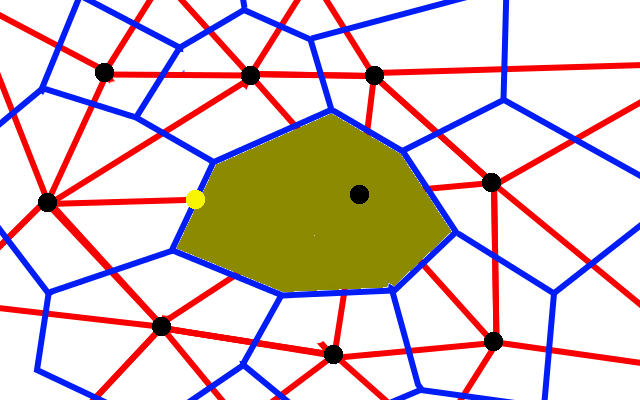
\includegraphics[width=\linewidth]{voronoi-churn4}
    \caption{Here, a new node is joining the networks and has established that his position falls in the the yellow shaded Voronoi region.}
    \label{churnjoin}
\end{figure}


\begin{figure}
    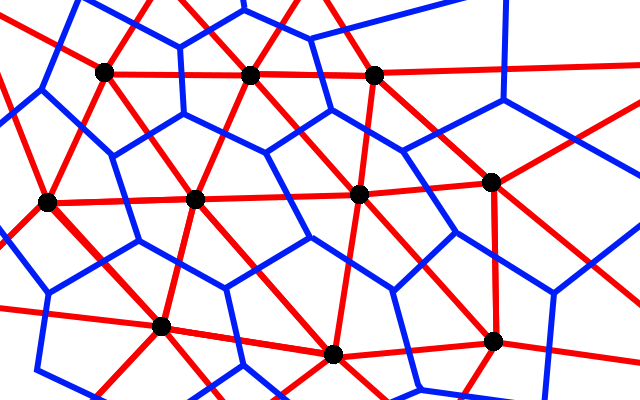
\includegraphics[width=\linewidth]{voronoi-example}
    \caption{The network topology after the new node has finished joining.}
    \label{churndone}
\end{figure}

\begin{figure}
    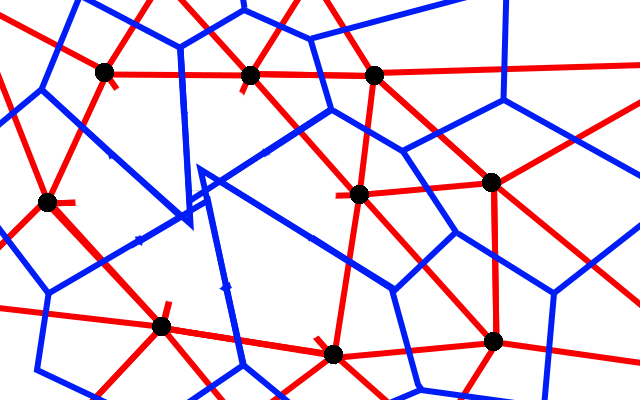
\includegraphics[width=\linewidth]{voronoi-churn1}
    \caption{The topology immediately after the new node leaves the network. After maintenance takes place, the topology repairs itself back to the configuration shown in Figure \ref{churninit}.}
    \label{churndrop}
\end{figure}


\subsection{Data Storage and Backups}
The primary goal of a DHT is to provide a distributed storage medium. We extend this idea to distribute work and information among nodes using the same paradigm. Resources in the network, be it raw data or assigned tasks, are assigned hash locations. The node responsible for a given hash location is responsible for the maintenance of that resource. When a node fails, its peers take responsibility of its space. Thus it is important to provide peers with frequent backups of a node's assigned resources.  That way, when a node fails, its peers can immediately assume its responsibilities.

When a resource is to be stored on the network, it is assigned a hash location. The hash locations assigned could be random, a hash of an identifier, or have specific meaning for an embedding problem. The node responsible for that resource's hash location stores the resource.

A resource is accessed by contacting the node responsible for the resource.  However, the requester generally has no idea which node is responsible for any particular resource.  The data request messsage is addressed to the location corresponding to the resource, rather than the node responsible for that location.  The message is forwarded over the overlay network, each hop bringing the node closer until it reaches the responsible node, who sends the resource or an error if the resource does not exist.

Some options are immediately apparent for dealing with wasted storage space. A system that is primarily read driven can record the time of the last read or a frequency of reads such that resources that are not read often enough are deleted after a certain period of time. If a system is write driven, allow the resource to be assigned a time to live, which can be updated as needed.

A node periodically sends a message containing backups of the resources for which it became newly responsible for to each of its peers. To minimize bandwidth and time wasted by backups, the node should only send the records changed since last backup.



\section{Implementation}
This section describes how the components of the D$^3$NS system piece together as a coherent whole.  We demonstrate how this system would be used in the real world to provide a better Domain Name Service.


\subsection{Establishment of a New Domain}
Under the current DNS system, a new domain name is purchased from a company registered with the Internet Corporation for Assigned Names and Numbers (ICANN). That company adds the domain name and a record provided by the owner to the TLD servers. The owner or management company then maintains a name server to answer DNS requests for the purchased domain. In D$^{3}$NS, new domain names are instead awarded as part of the blockchain mining process or purchased from a previous owner, then transferred to the new owner. These assignments and transfers are both recorded in the blockchain. 

A prospective domain owner can use their own mining software and mine a domain name or purchase a domain name voucher from a miner and exchange it for a domain name. In the blockchain, domain name owners are referred to by their public key. The public key is used to authenticate both records and transfers of domains. Loss of the private key of an account will result in the loss of ability to update DNS records and the ability to transfer the domain. 


\subsection{Updating Records for a Domain}
A domain name record in the current DNS system is used to indicate a record on your own Name Server or to configure the record held by the TLD server that contains the address record. Using D$^3$NS, all records must be signed using their owner's private key and confirmed with the public key. 

A properly configured D$^3$NS server should not accept any DNS records which have not been signed by their owner or accept a record with an older version number. To push a new DNS record for a domain, the owner must create the record set for the domain and then sign and submit it to a node on the DHT. The DHT will forward the record to the responsible party and store it after confirming its validation. The new record will begin to be broadcast to clients after old records begin to expire and caches seek new records.

\subsection{Looking up a DNS record}
In the current DNS configuration, a record is looked up using a UDP system that queries a tree of servers. clients send queries to  a local DNS server which acts as a DNS resolver and cache. If a portion of the domain name is unknown, the resolver sends a request to the responsible server and looks the record up recursively.

This system is largely unchanged under D$^{3}$NS from the point of view of the DNS resolver and client. Ideally, the resolver or client has chosen a nearby member of the D$^{3}$NS network as its root domain name server (it can also maintain a large list of backup servers, should the current one fail). The resolver requests a domain's record from the D$^{3}$NS node. The node then forwards the request to the responsible party. If any node along the route has a valid cache of the required record, then that server responds and routes the message back to the entry node. All nodes along the route cache the response to aid future queries.

\subsection{Caching}
DNS needs to aggressively cache lookups. Previous investigations into optimizing caching on a DHT saw favorable results \cite{irm}. However, with the specific application of DNS in mind, the time-to-live field on DNS records defer the caching optimization problem onto users. 
While it may be tempting to utilize the built in time-to-live field for caching on the DHT, the possible cyclical nature of cache passing may result in difficulty in propagating new records.

 
Integrated File Replication and Consistency Maintenance (IRM) \cite{irm} views the process of caching and keeping the cache up to date as components of larger problem.  Nodes in the DHT keep track of how often records are requested and cache those records once a defined rate is passed.  Nodes then request an update for the cache based on how often the record is requested and how often that request is expected to be changed by the owner.


In the current implementation of DNS, caching involves a time-to-live field defined by the domain owner. This means that no effective cache optimization done by the server; rather the server that trusts records to have a sensible time-to-live value. IRM \cite{irm} can be used to approximate the correct time-to-live value for a record.

\section{Conclusion and Future Work}
D$^3$NS was successfully implemented to act as a DNS server.  A user would query the a computer we set up as a DNS gateway which was a member of the DHT and mining network. If the queried domain had a record stored in the DHT and an owner established in the blockchain, the server would reply with the stored DNS records. Otherwise the server would reply with a DNS failure. We ran the DHT and mining network on a cluster of computers and an artificially low difficulty such that a live demo of mining would be viable.

Using all of these components together allowed us to create a system with the following features:
\begin{itemize}
	\item Robustness - The DHT and Blockchain are both robust to failures and attacks.
	\item Extensibility - The DNS reverse compatibility allows any DNS extension to be utilized, if dynamic resolution is required a name server record can be stored in the DHT to point to a user's specialized DNS servers.
	\item Decentralization - Both the DHT and Blockchain can operate without the support of any controlling organization, this offers security against corruption and abuse. 
\end{itemize}	

D$^3$NS successfully addresses the challenges laid down by Cox et al \cite{cox}  in regards to designing a DNS replacement running over a DHT.   We encourage criticism, revision, and adoption of this new system.

\subsection{Unaddressed Issues and Future Work}
The Blockchain does not solve all security issues relevant to DNS authentication and security. Exit nodes could lie or have packets inject to clients until the protocol from DNS server to client is improved. The DHT structure opens up unexplored disruption attacks on the overlay topology.

A series of issues relevant to VHash are not addressed in this paper due to limiting of scope, space, time, and a lack of actual solutions to the problems: The exact method of caching to optimize lookup time under real world usage. The overlay network being mapped onto latency results in nodes whose failure due to natural disaster to be comorbid with it's neighbors resulting to data loss. Comorbidity could be counteracted by more complex backup schemes.

Future work will explore various solutions to theses issues, as well as generalized improvements to D$^3$NS as whole.  In particular, the technique of allying a DHT value store for real-time data and a Blockchain for ownership verification may prove a viable technique for decentralizing other web services and enabling new shared storage and computation mediums.


\bibliographystyle{ieeetr}
\bibliography{P3DNS}
\end{document}
